\section{Base-model evaluation}
\label{sec:evaluation}

All numbers below are 0-shot lm-eval results for the step-700k
checkpoint unless marked otherwise; reference models are quoted at their
published settings.

\begin{table}[h]
\centering
\small
\caption{0-shot suite at step 700k, against same-class references.
``prev gen'' is this project's predecessor campaign (337M, 40B
tokens, 128k-vocab tokenizer).}
\label{tab:evals}
\begin{tabular}{lcccccc}
\toprule
task & \textbf{ours} & SmolLM2 & SmolLM & Qwen2.5 & Gemma3 PT & prev gen \\
 & 308M / 0.37T & 360M / 4T & 360M / 0.6T & 0.5B & 270M & 337M / 40B \\
\midrule
HellaSwag & \textbf{56.9} & 54.5 & 51.8 & 51.2 & 40.9 & 50.6 \\
ARC avg & \textbf{53.8} & 53.0 & 50.1 & 45.4 & 43.4 & 48.9 \\
PIQA & \textbf{75.2} & 71.7 & 71.6 & 69.9 & 67.7 & 72.1 \\
OpenBookQA & \textbf{38.8} & 37.4 & 37.2 & 37.4 & --- & 36.2 \\
BoolQ & 58.0 & --- & --- & --- & 61.4 & 60.1 \\
\midrule
Lambada & 47.4 & \multicolumn{5}{l}{SciQ 92.0 \quad COPA 72.0 \quad
ARC-e/c 67.5 / 40.1} \\
\bottomrule
\end{tabular}
\end{table}

\begin{figure}[t]
\centering
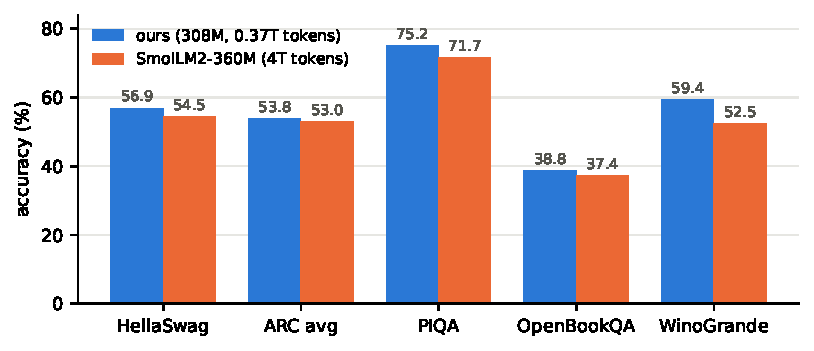
\includegraphics[width=0.9\textwidth]{figures/eval_bars.pdf}
\caption{Ours vs.\ the strongest same-size reference. The model is
ahead on every comparable row while having seen $\sim$1/11 the
pretraining tokens.}
\label{fig:evalbars}
\end{figure}

The headline is the data efficiency: the model beats SmolLM2-360M ---
the strongest same-size open reference, trained on 4T tokens --- on
every row where the numbers are comparable, from an 11$\times$ smaller
token budget. Three further panels complete the picture:

\begin{table}[h]
\centering
\small
\caption{Post-hoc loglikelihood and generation panels (step 700k).}
\label{tab:panels}
\begin{tabular}{llll}
\toprule
task & ours & best same-class reference & note \\
\midrule
WinoGrande 0-shot & \textbf{59.4} & SmolLM-360M 52.8 & $+5$ over every reference \\
WinoGrande 5-shot & \textbf{57.9} & Qwen2.5-0.5B 54.1 & \\
MMLU cloze 0-shot & 30.0 & SmolLM2-360M 35.8 & between SmolLM 135M/360M tiers \\
TriviaQA 5-shot & 15.3 & SmolLM2-360M 16.9 & parity with Gemma3 PT (15.4) \\
GSM8K 5-shot & 1.1 & SmolLM2-360M 3.2 & base-model band, pre-SFT \\
\bottomrule
\end{tabular}
\end{table}

WinoGrande is the standout --- $+5$ points over every reference on a
task where this size class barely clears chance --- and, with HellaSwag
and PIQA, suggests the architecture's strength is concentrated in
commonsense/coreference resolution. The two knowledge-bound scores
(MMLU cloze, TriviaQA) track factual \emph{exposure} rather than
capability and sit where an 0.37T-token diet predicts: this is the axis
post-training distillation from a knowledge-rich teacher targets next.
CommonsenseQA in standard format scores 26.2; small base models cluster
at chance there, and published references using cloze formulations are
not comparable.
